В нашем проекте Zabbix был использован для: 
\begin{itemize} 
\item мониторинга состояния сети; 
\item контролирование ресурсов сервера.
\end{itemize} 

Была проделана следующая работа: 
\begin{itemize} 
\item был установлен и настроен Zabbix-сервер; 
\item для роутера и свитча были написаны шаблоны для получения данных по SNMP; 
\item для сервера был установлен и настроен Zabbix-агент, для получения данных с агента используется стандартный шаблон. 
\end{itemize} 

\begin{figure}[ht!] 
\center{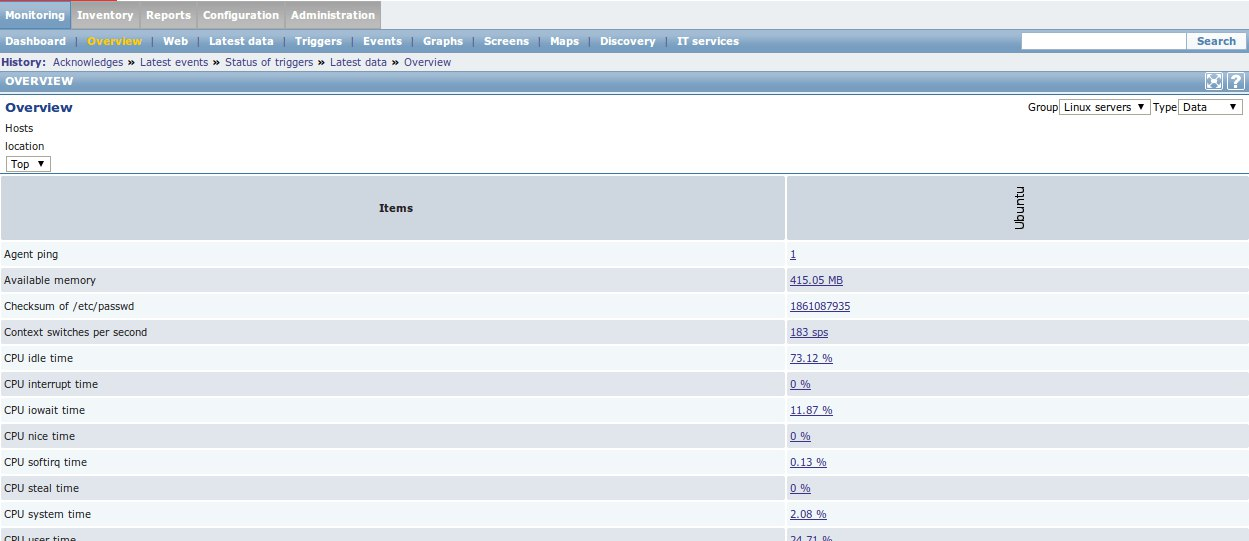
\includegraphics[width=0.8\linewidth]{eco/images/zbx.jpg}} 
\caption{Просмотр данных о сервере} 
\end{figure} 

Работа над шаблонами: 
\begin{itemize} 
\item Для начала были получены с устройств строки OID; 
\item Для каждой строки OID было написано правило обнаружения в шаблоне; 
\item Далее создавались элементы данных и триггеры; 
\item Были созданы несколько графиков. 

\begin{figure}[ht!] 
\center{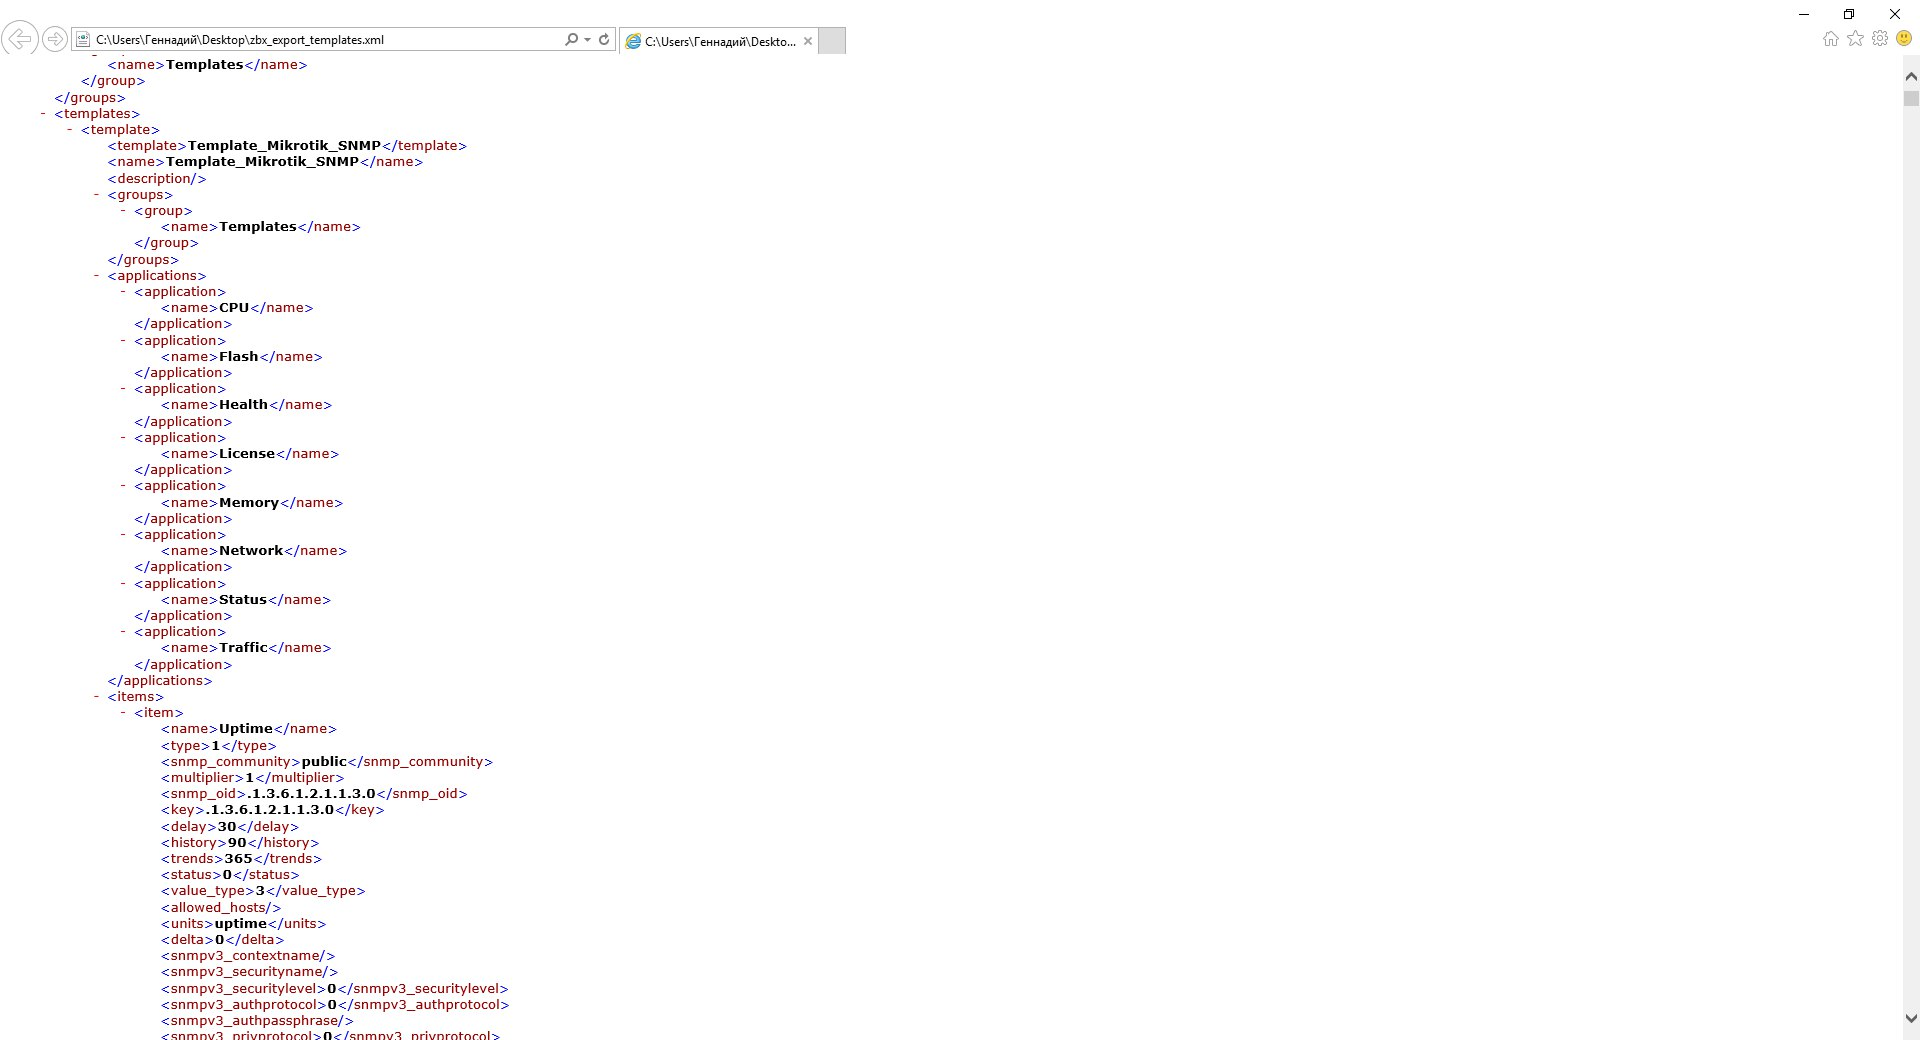
\includegraphics[width=0.8\linewidth]{eco/images/gena_zabbix.jpg}} 
\caption{Пример готового шаблона} 
\end{figure}